\documentclass[11pt]{article}

\usepackage{graphicx}
\usepackage{float}
\usepackage{listings}
\usepackage{amsfonts} 
\usepackage{amssymb}
\usepackage{longtable}

\usepackage[no-math]{fontspec} 
\setmainfont{Times New Roman}

\usepackage{hyperref}
\hypersetup{
    colorlinks=true,
    linkcolor=blue,
    filecolor=magenta,      
    urlcolor=cyan,
}

\newcommand{\classname}[1]{\textit{\textbf{#1}}}
\newcommand{\varname}[1]{\underline{\textit{#1}}}
\newcommand{\funcname}[1]{\textit{#1}}

\title{ICS2211 Assignment}
\author{Lorenzo Catania (Team \#8, life below water)}

\begin{document}

\maketitle

{
  \hypersetup{linkcolor=black}
  \tableofcontents
}

\section{Introduction}
\subsection{Game concept}
The presented project is a simil-arcade game called \textbf{Deep Blue}, set in a fictionary submarine world where fishes became so used to the garbage dumped in the ocean that they genetically mutated and started eating it.
You embody a scuba diver that has to collect as much rubbish as possible while being chased by mutant sea creatures.

\subsection{Game mechanics}
The game is a side-scroller runner where the world is discovered from left to right, with the camera moving accordingly.
The player has to collect as much garbage items (represented by cans, plastic bags, plastic bottles etc...) to increase its score.
Foes are spawned and will start patrolling different areas of the screen. If the player stays for a consistent time close enough to an enemy then it starts chasing and attacking the character. The player has no way to counterattack, its aim is to run away from fishes (they'll disappear completely after falling out of the left side of the camera).

The player must also take care of the oxygen available, that goes down while being underwater and can be recharged going back to the surface level. The oxygen drops faster based on the depth the character is on.
If the oxygen finishes, the player starts losing health.

It's possible to find some power-ups on the map or into trash items.
Those are useful to heal, recover oxygen or permanently increase the character's speed to make it easier to run away from enemies.

The environment is procedurally generated, meaning that each game may be potentially infinite. Items, collectables and enemies are spawned randomly on the right and are automatically garbage-collected when falling over the left of the screen.
The enemies strength grows over time and there's a little chance that an enemy evolves to a more dangerous kind of organism.

\section{Software architecture}
\subsection{Development environment}
The game has been developed using Unity3D 2018.4.13f and the game has been tested on both Windows and GNU/Linux operating systems. No specific versioning control software has been used, but it's possible to reconstruct a rough history of the code because each proposed change was packaged into a Unity Package and imported by the rest of the team after it was tested accurately.

\subsection{Components}
\subsubsection{Level generation}
The LevelGenerator is responsible for spawning collectables and in general any neutral entity the player can interact with.
It contains a list of prefabs with the respective probability of spawning and the range of coordinates they can appear into.
The level generation happens on an area placed on the right side of the camera that's still not visible to the player.
This area is splitted into tiles of fixed size and it's periodically filled with entities that are then attached to the root node of the scene so they can shift on the left and interact with the current game environment. Two entities spawned in the same update can't appear in near tiles to guarantee world variety.
Note that enemies could be spawned by level generator, but they're not in the final version of the game because a more dynamic way of evolving has been preferred. In fact, game objects spawned by level generator are initialized in-place and just deallocated when their cycle of life finishes. This approach doesn't affect performances for simple objects, but may limit the versatility of highly "intelligent" ones like enemies.

\begin{figure}[H]
  \centering
  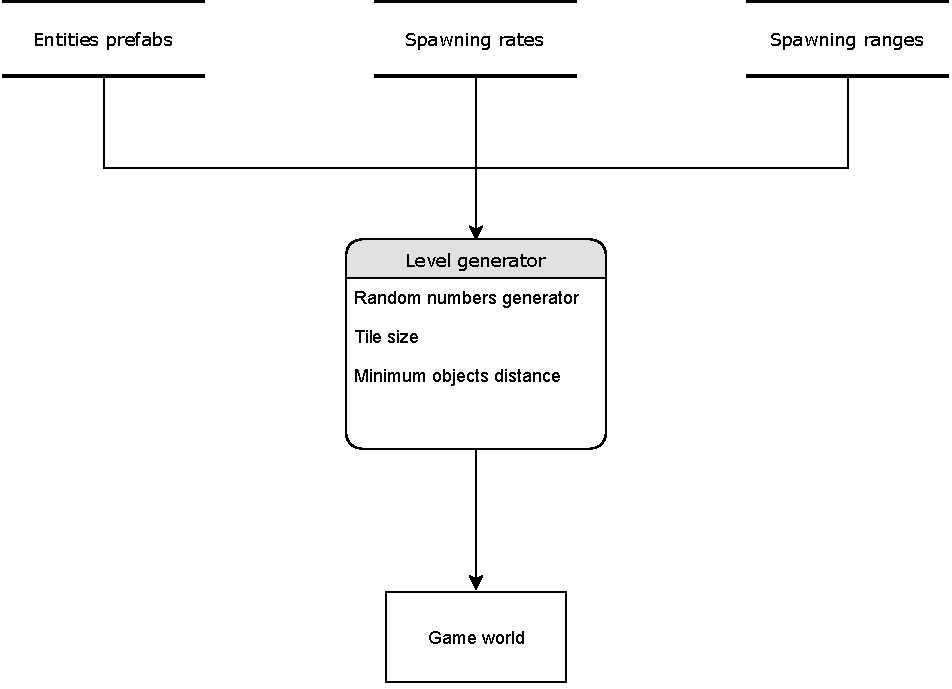
\includegraphics[width=1.0\textwidth]{figures/level_generator}
  \caption{Level generation data flow}
\end{figure}

\subsubsection{Camera movement control}
The CameraController component handles the main camera movement and the appearance of visual details in the scene.

The camera smoothly follows the player movement, but it's clamped on the vertical axis to avoid showing the void behind the background sprite. The camera moves slightly faster on the horizontal axis based on how close is the player to the right bound of the screen.

As the player object actually moves in the scene world, the background image must be continously shown and moved towards, without allowing the user to notice the loop and break the magic.

Two seamless background textures are loaded and put side by side. When the leftmost one remains out of camera visual, it's translated on the right of the other and so on.
Doing so the player will never see the void behind the background and performances won't be affected too much as the only operation done is a casual translation.

\begin{figure}[H]
  \centering
  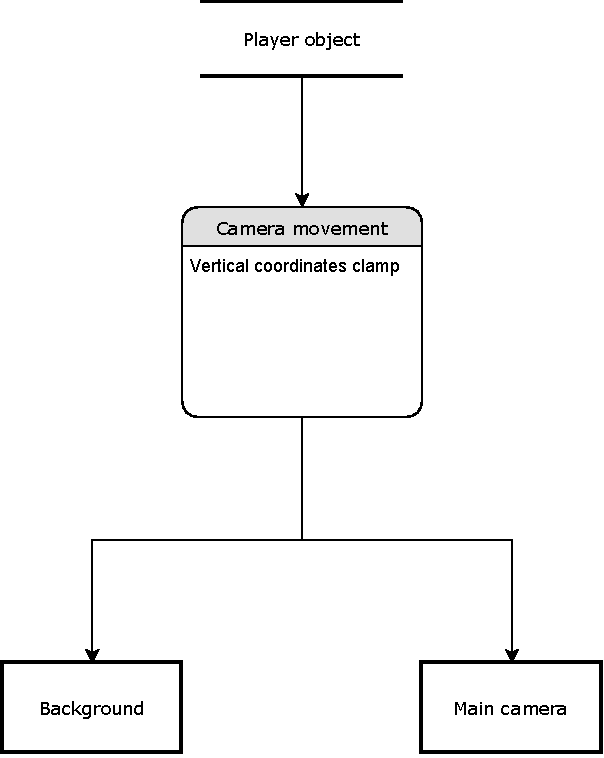
\includegraphics[width=0.8\textwidth]{figures/camera_controller}
  \caption{Camera control data flow}
\end{figure}

\subsubsection{Player control}
The player object is controlled using the mouse. The movement is smoothed based on how far is the mouse pointer and the rotation is not sudden as well to simulate a visual underwater physics effect. Furthermore, the head movement is faster than the body movement and tends to follow the mouse pointer much faster to give a better idea of where the player will go.

Player's health and oxygen values are handled by a script as well, mainly to determine the game over. External entities interactions (enemies, collectables etc...) may change those values as well.
The player position is checked on every update loop to determine whenever oxygen is gained or spent based on the depth (represented by its position in the Y axis).

Raycasting is used all around the player object to see if any collectable is present and in case there is to pick it up.

\begin{figure}[H]
  \centering
  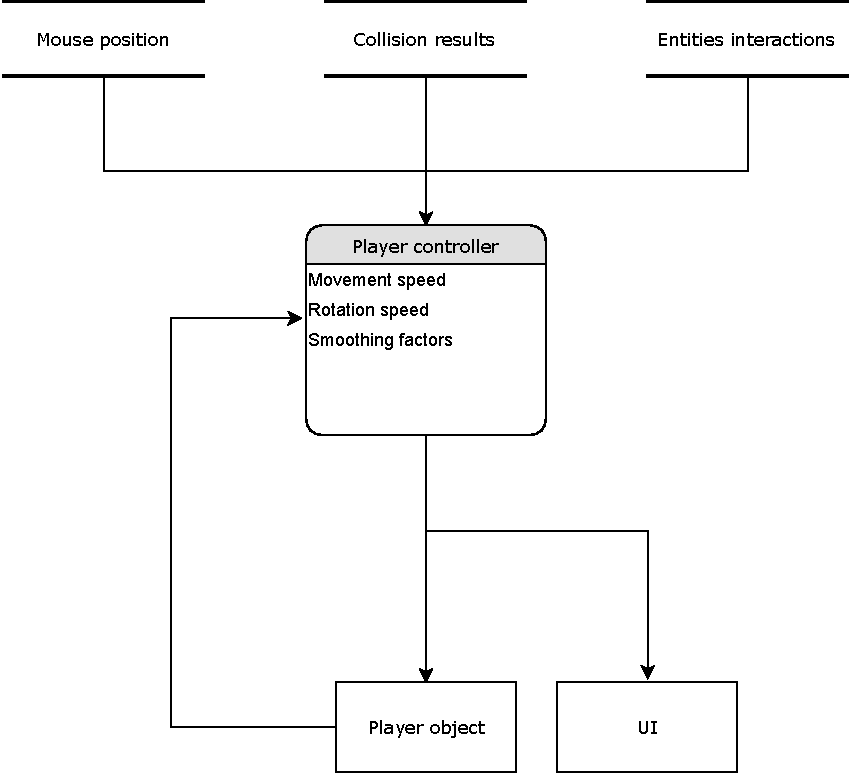
\includegraphics[width=1.0\textwidth]{figures/player_controller}
  \caption{Player control data flow}
\end{figure}

The backward arrow between the player object and its controller represents the usage of current player data (for example, the position) to compute what the values should be present in the next step.

\subsubsection{Entities garbage collection}
A "death wall" object is placed on the left of the screen and it moves following the camera. It has a trigger that collides with all the game objects (expect the background sprites). Each time an object is far enough from the user's point of view it gets deleted or sent back to its relative pool to optimize memory usage and clean up the scene from useless objects that shouldn't be rendered anymore.

\subsubsection{Game state and UI}
In the current version, the game state is given only by the score. A \textit{ScoreManager} is used to take track of its value and to update the score's label on the GUI.

Menus are composed by simple buttons that interact with a \textit{ButtonHandler}, calling different function based on what action must be executed (most of the time they load a different scene).
In-game user interface is made of icons and sliders or texts that represents the player stats and the current user score. They're updated by controller as well.

\subsubsection{Enemies spawning}
Model used to spawn enemies in the game world is unique and tuned specifically for gradually increasing the match difficulty.
It's based on a genetic algorithm, applied to a pool of pre-instantiated enemy objects that are partially destroyed and initialized again during the breeding phase.

Enemies in the pool are breeded periodically, while a new enemy is popped out from the pool and spawned in the world once in a while. Note that enemies currently present in the scene are not involved in breeding, so the process is completely invisible to the user.

Different kind of enemies can be encountered while playing and the variety is guaranteed by mutations during reproduction on fishes, meaning that a child may mutate to a different species instead of inherating its genes from the parents. The chance of encountering weaker species decreases over time.

The approach used to breed enemies is described in details in the next section.

\begin{figure}[H]
  \centering
  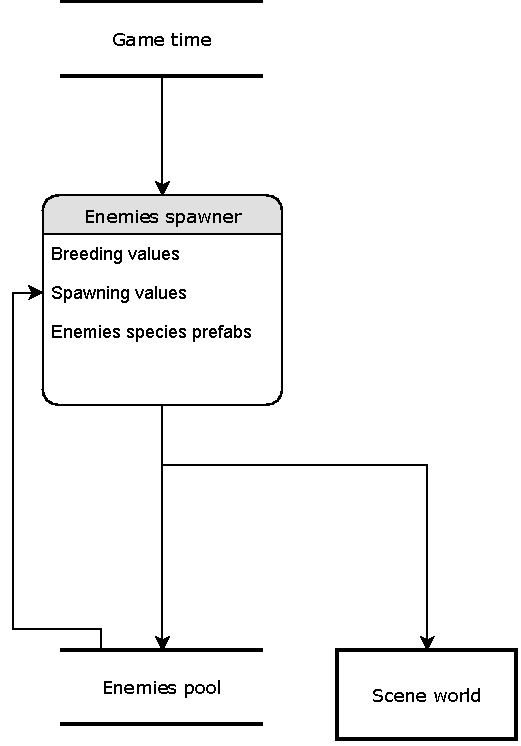
\includegraphics[width=0.6\textwidth]{figures/enemies_spawner}
  \caption{Enemies spawner data flow}
\end{figure}

\section{Artificial Intelligence features}
\subsection{Enemies behaviour state machine}
The enemies behaviour is traced by a simple finite state machine that contains two states: \classname{patrolling} and \classname{attack}.

\begin{figure}[H]
  \centering
  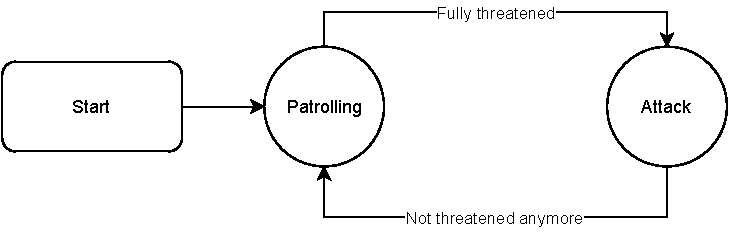
\includegraphics[width=0.6\textwidth]{figures/enemy_behaviour_states}
  \caption{Enemy behaviour state machine}
\end{figure}

Transitions between those two states are triggered by a single variable \varname{threat}. The threat level increases and decreases based on how far the player is from an enemy and for how much time.

Threating is based on a fuzzy system, defined by the \varname{threat} value itself, \varname{onAlertThreshold} and \varname{attackThreshold}.

\begin{figure}[H]
  \centering
  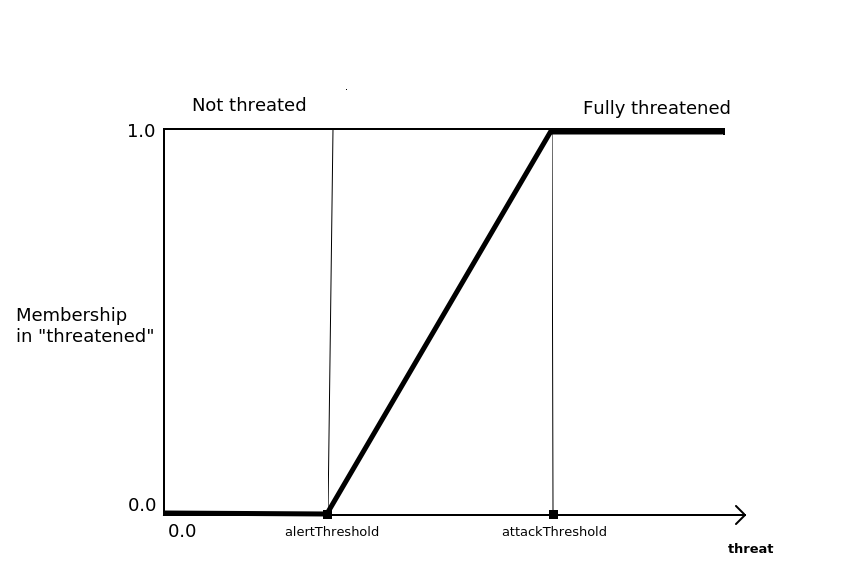
\includegraphics[width=0.8\textwidth]{figures/threat_graph}
  \caption{Threatening evaluation graph}
\end{figure}

As the \varname{threat} value grows, the enemy is first on guard and then starts attacking. When \varname{threat} value goes down, the enemy stops chasing and keeps patrolling again.

Note that if $alertThreshold < threat < attackThreshold$ the enemy's behaviour state doesn't change. While in this level, the enemy keeps doing the same thing it was doing until one of the threshold is hit.

\begin{lstlisting}
  procedure PatrolBehaviourUpdate():
    PatrolArea() // Moves randomly around the current position

    if threat > attackThreshold:
      SetState(Attack)
\end{lstlisting}

\begin{lstlisting}[language=C]
  procedure AttackBehaviourUpdate():
    ChaseEntity(playerObject) // Moves towards the player

    // If close enough to the player, attack him and reduce its HP
    if CloseTo(playerObject) and attackCooldown == 0: 
      Attack(playerObject)

    if threat < alertThreshold: 
      SetState(patrol)
\end{lstlisting}



\end{document}